\documentclass[12pt,a4paper]{article}

\usepackage{allrunes}
\usepackage{amsmath}
\usepackage[magyar]{babel}
\usepackage[T1]{fontenc}
\usepackage[utf8]{inputenc}
\usepackage{fixltx2e}
\usepackage{multirow}
\usepackage{hyperref}
\usepackage{amsfonts}
\usepackage{amsthm}
\usepackage{amssymb}
\usepackage{indentfirst}
\usepackage{listings}
\usepackage{color}

\definecolor{mygray}{rgb}{0.4,0.4,0.4}
\definecolor{mygreen}{rgb}{0,0.8,0.6}
\definecolor{myorange}{rgb}{1.0,0.4,0}

\lstset{
basicstyle=\footnotesize\sffamily\color{black},
commentstyle=\color{mygray},
frame=single,
numbers=left,
numbersep=5pt,
numberstyle=\tiny\color{mygray},
keywordstyle=\color{mygreen},
showspaces=false,
showstringspaces=false,
stringstyle=\color{myorange},
tabsize=2
}

\usepackage[a4paper]{geometry}

\geometry{a4paper,
		     tmargin = 35mm, 
		     lmargin = 25mm,
		     rmargin = 30mm,
		     bmargin = 30mm}

\theoremstyle{plain}
\usepackage{graphicx}

\usepackage{float}
\renewcommand\thesection{\Roman{section}}

\title{\textbf{3rd report}}

\author{\Large{\textsc{Alex Olar}} \vspace{10pt}\\
	\textrm{University of Eötvös Loránd}
	}
\date{}

\begin{document}

\maketitle

\par This week I updated my plotting code significantly. I ran the code
with different types of fields, such as the stress field code-named ELTE and
several analytic fields. The analytic fields only differ in accuracy since they are
calculated using N \textbf{--WHAT--}.

\par The ELTE field looks the following way:

\begin{figure}[H]
	\centering
	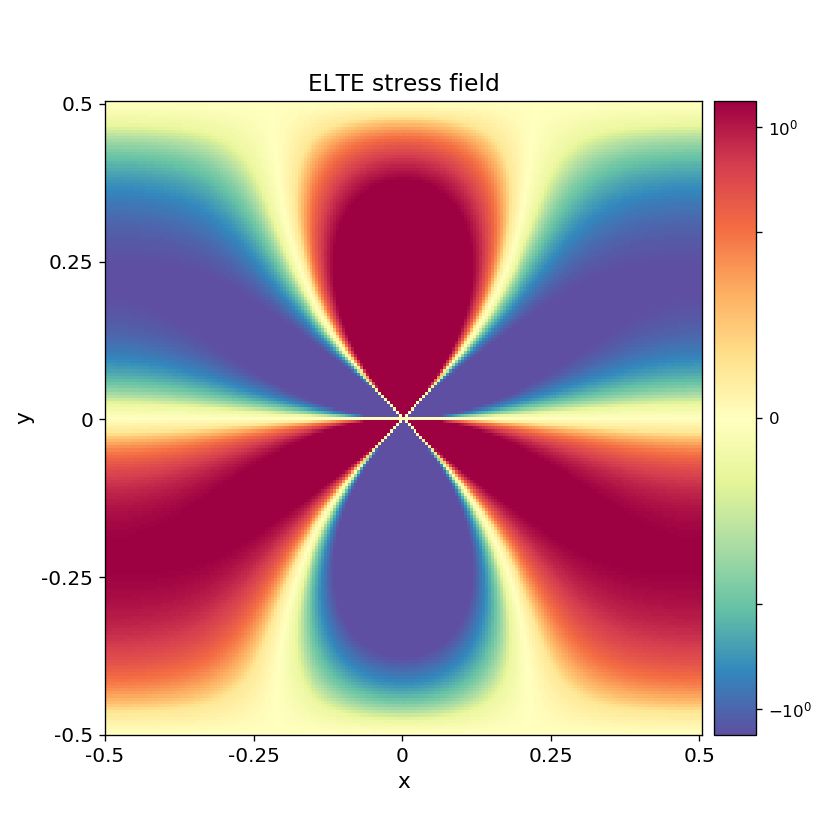
\includegraphics[width=0.5\textwidth]{../elte_stress_field.png}
\end{figure}

\par While changing N from 1 to 12 in the calculataion of analytic fields results are the
following in order:

\vspace{1cm}

\begin{minipage}{0.24\textwidth}
	\centering
	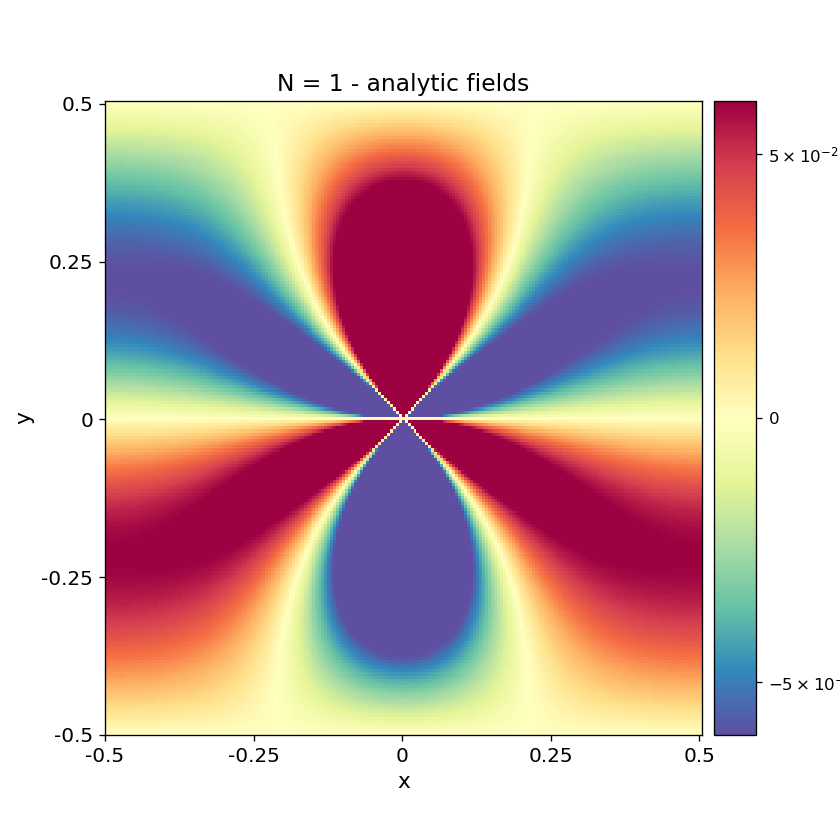
\includegraphics[width=\textwidth]{../stress_field_01.png}
\end{minipage}
\begin{minipage}{0.24\textwidth}
	\centering
	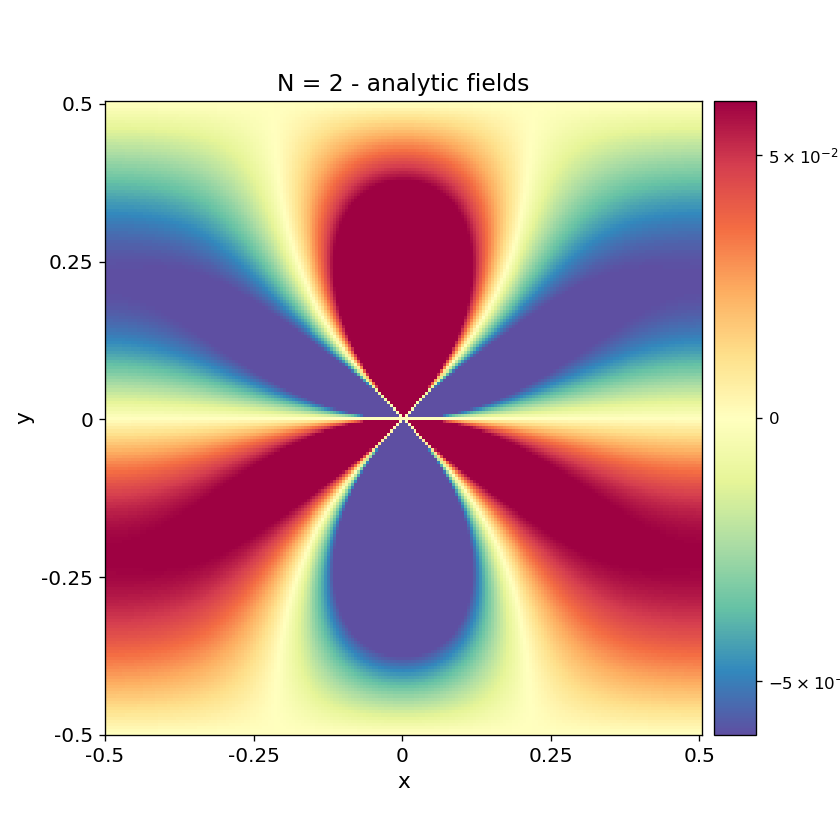
\includegraphics[width=\textwidth]{../stress_field_02.png}
\end{minipage}	
\begin{minipage}{0.24\textwidth}
	\centering
	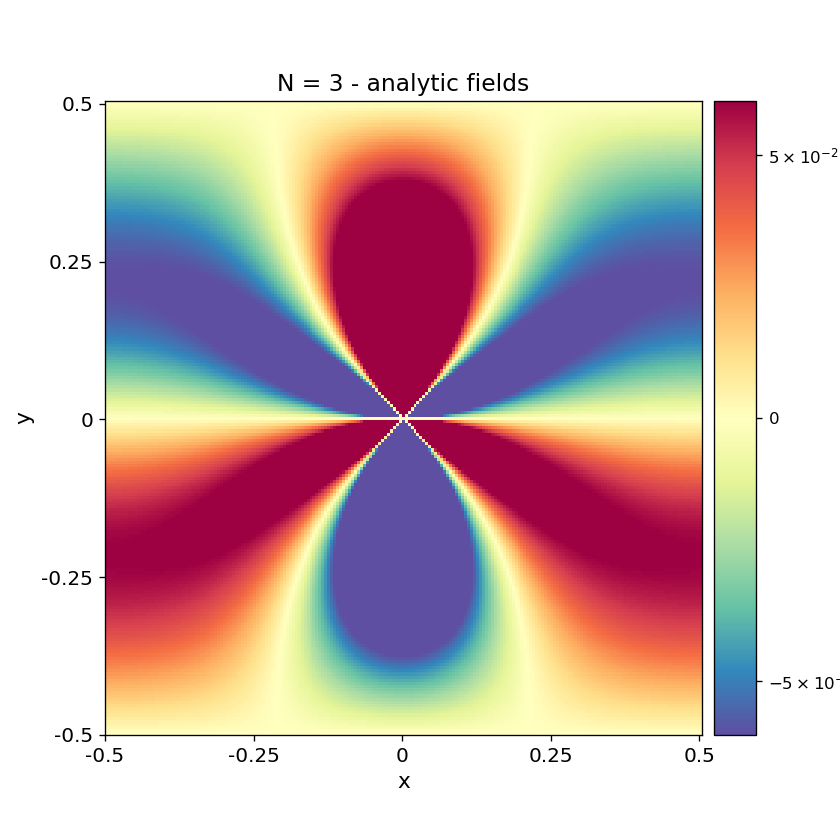
\includegraphics[width=\textwidth]{../stress_field_03.png}
\end{minipage}	
\begin{minipage}{0.24\textwidth}
	\centering
	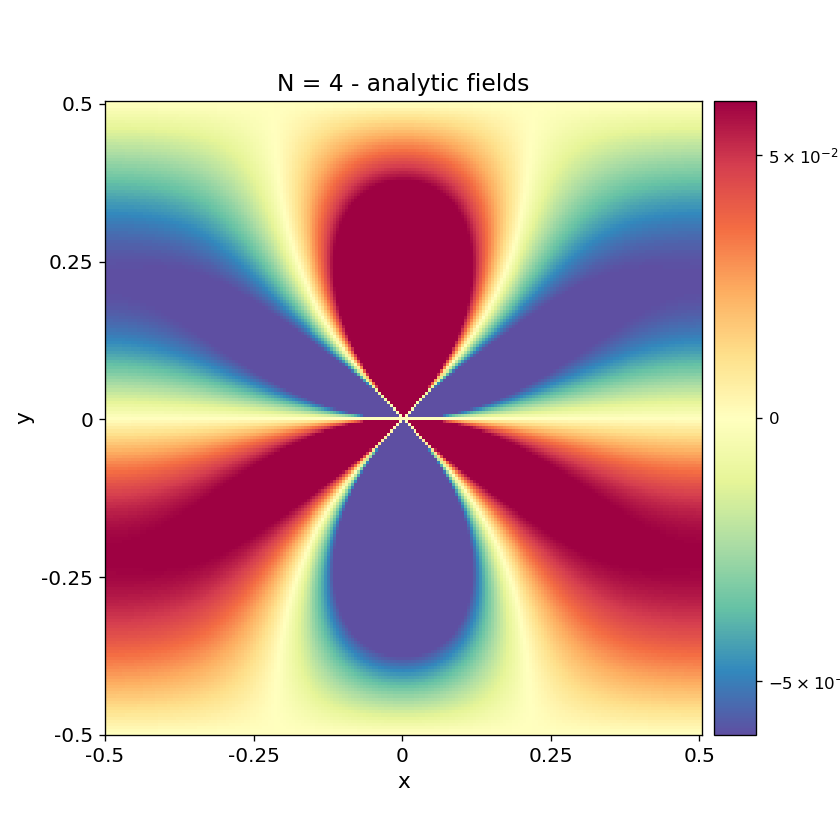
\includegraphics[width=\textwidth]{../stress_field_04.png}
\end{minipage}	

\begin{minipage}{0.24\textwidth}
	\centering
	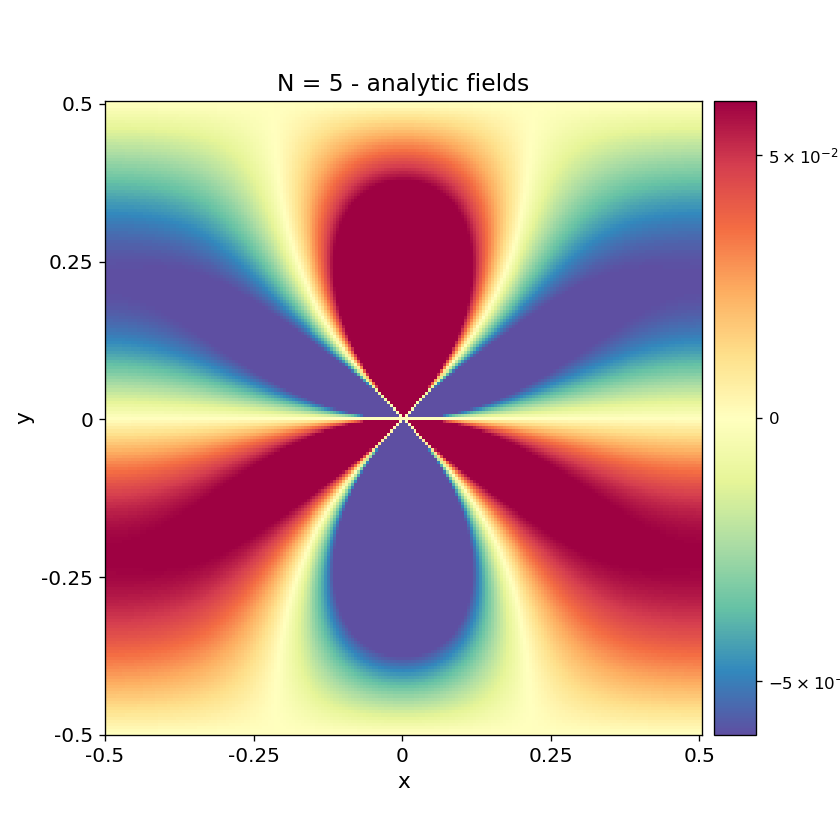
\includegraphics[width=\textwidth]{../stress_field_05.png}
\end{minipage}
\begin{minipage}{0.24\textwidth}
	\centering
	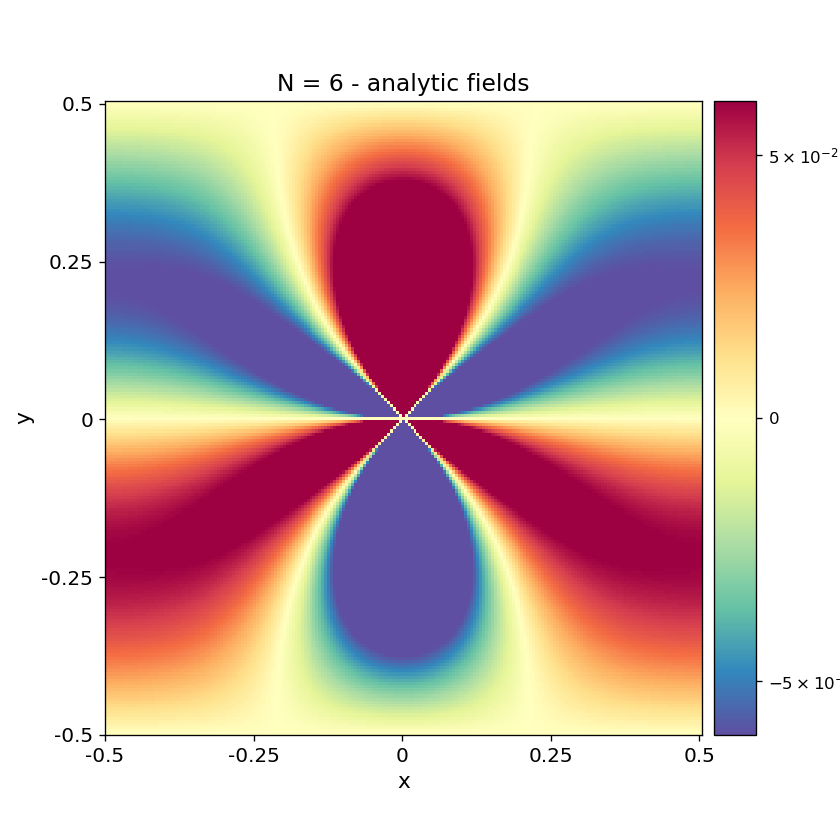
\includegraphics[width=\textwidth]{../stress_field_06.png}
\end{minipage}	
\begin{minipage}{0.24\textwidth}
	\centering
	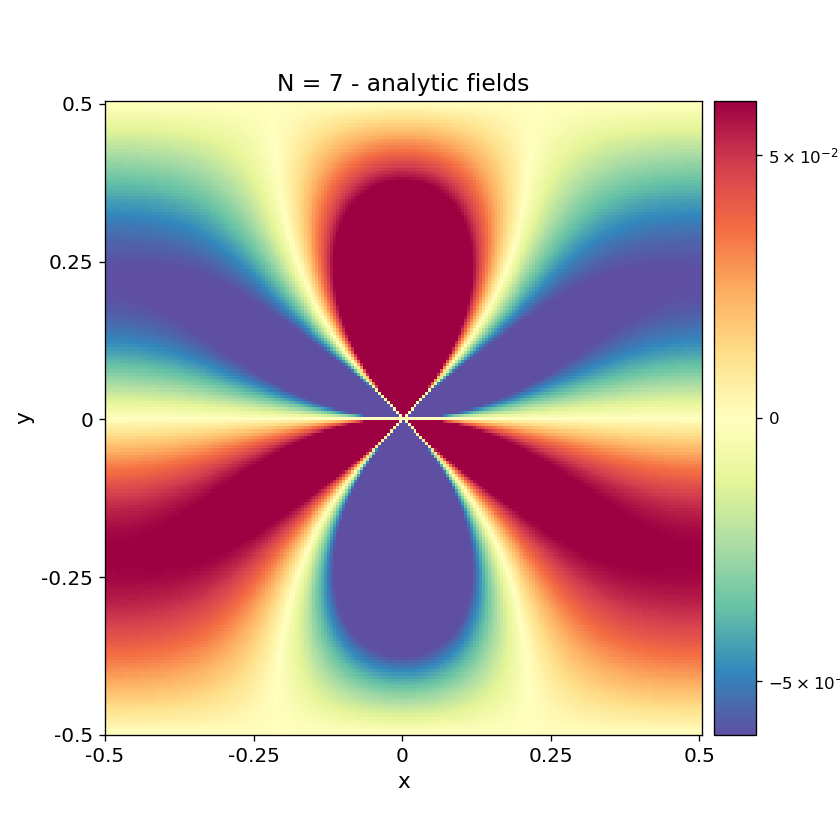
\includegraphics[width=\textwidth]{../stress_field_07.png}
\end{minipage}	
\begin{minipage}{0.24\textwidth}
	\centering
	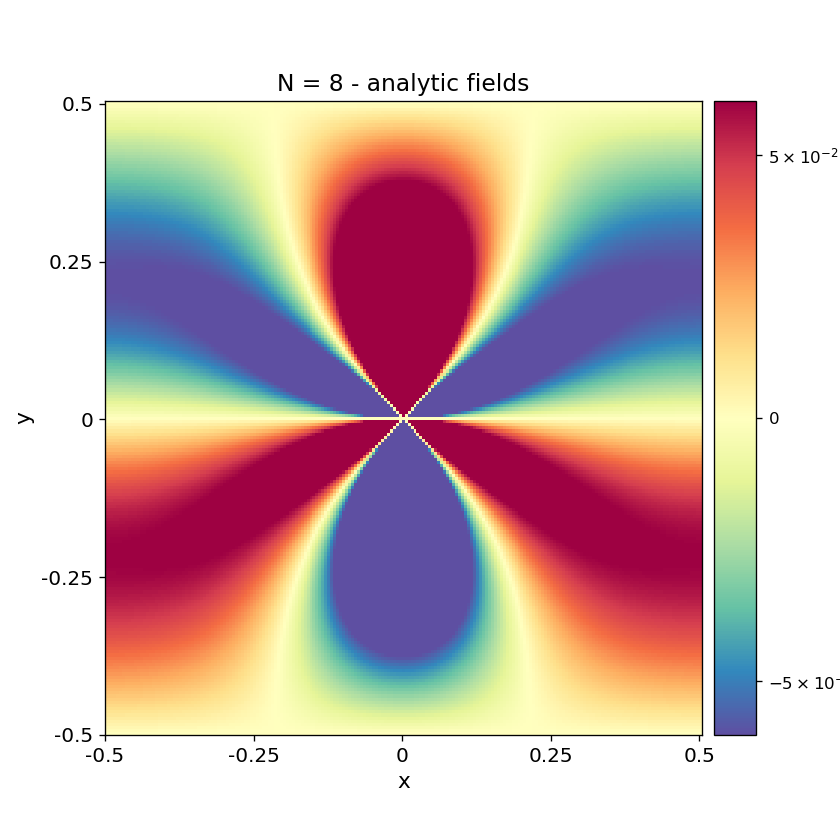
\includegraphics[width=\textwidth]{../stress_field_08.png}
\end{minipage}	

\begin{minipage}{0.24\textwidth}
	\centering
	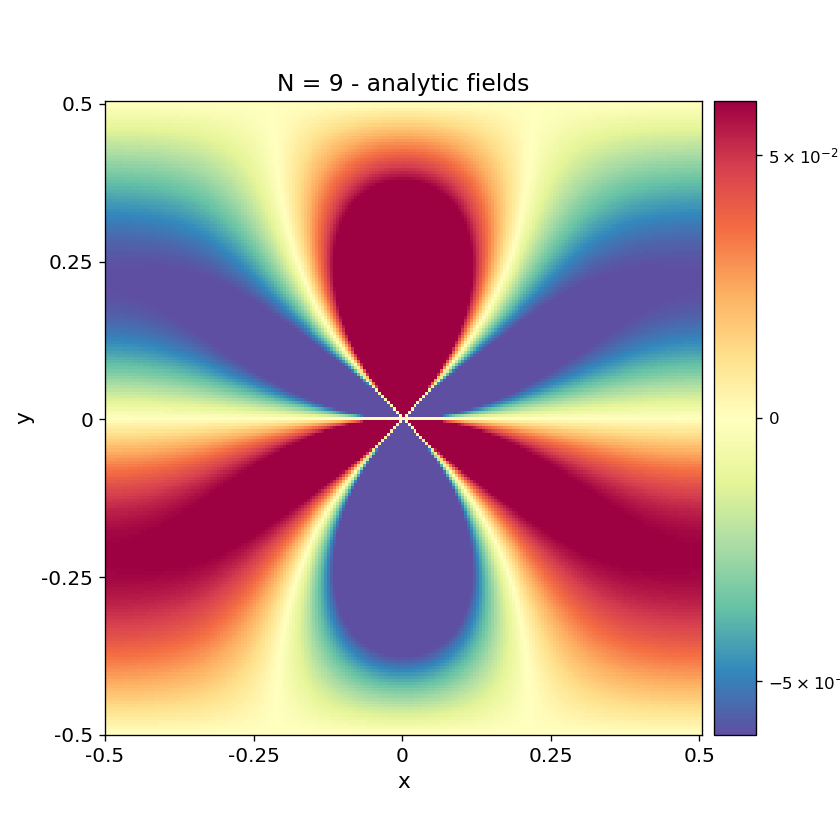
\includegraphics[width=\textwidth]{../stress_field_09.png}
\end{minipage}
\begin{minipage}{0.24\textwidth}
	\centering
	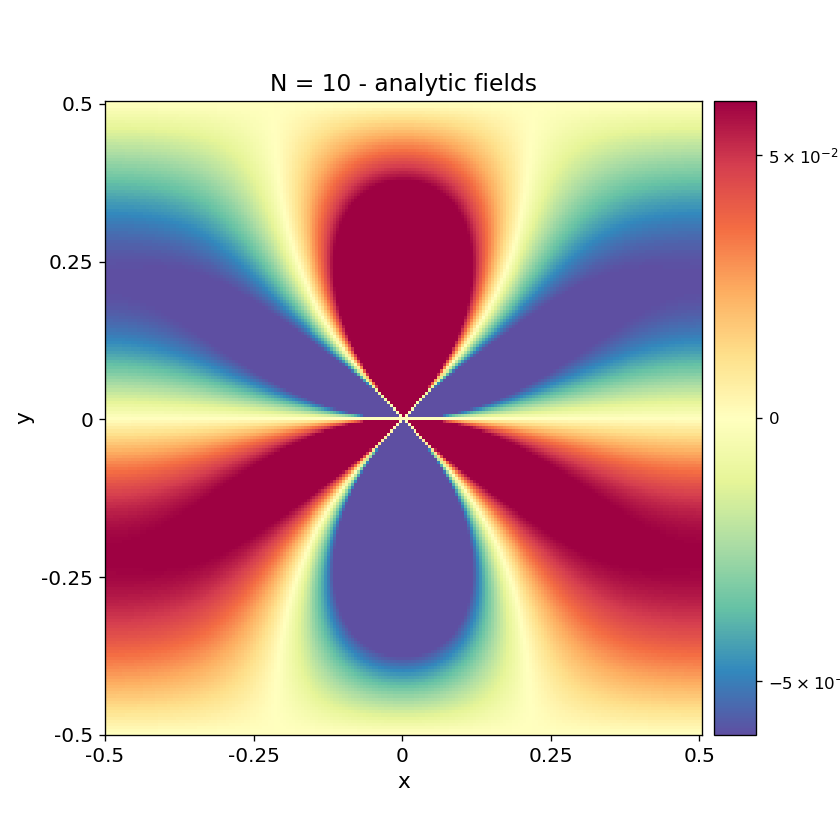
\includegraphics[width=\textwidth]{../stress_field_10.png}
\end{minipage}	
\begin{minipage}{0.24\textwidth}
	\centering
	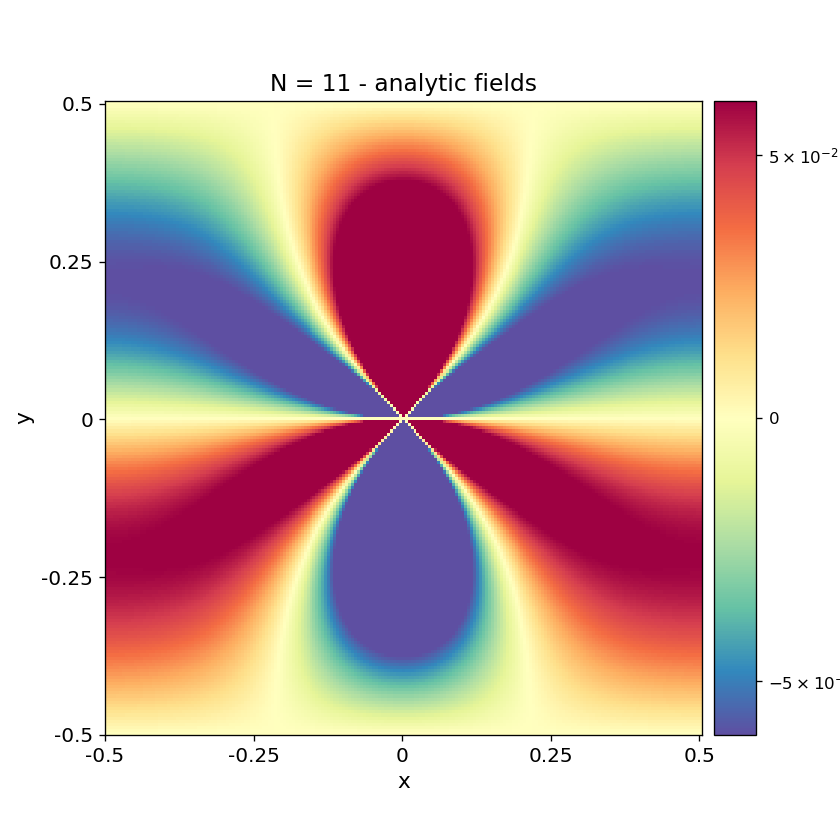
\includegraphics[width=\textwidth]{../stress_field_11.png}
\end{minipage}	
\begin{minipage}{0.24\textwidth}
	\centering
	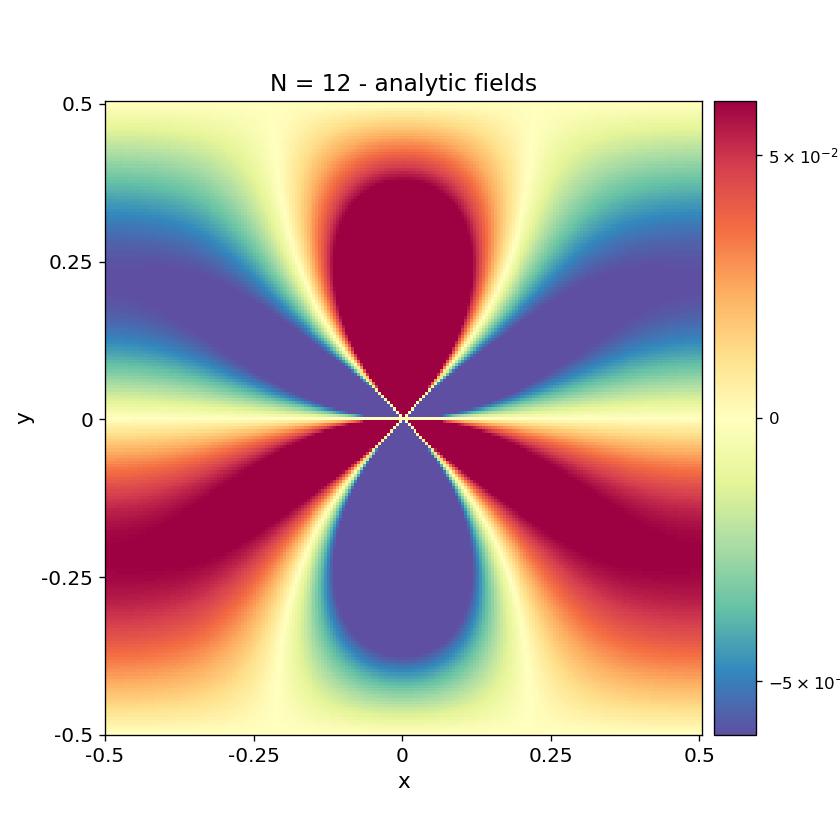
\includegraphics[width=\textwidth]{../stress_field_12.png}
\end{minipage}

\vspace{1cm}

\par The difference doesn't really show on the images but getting the
consecutive differences of images and displaying that one can achive
much better visualization of the fields:

\begin{figure}[H]
	\centering
	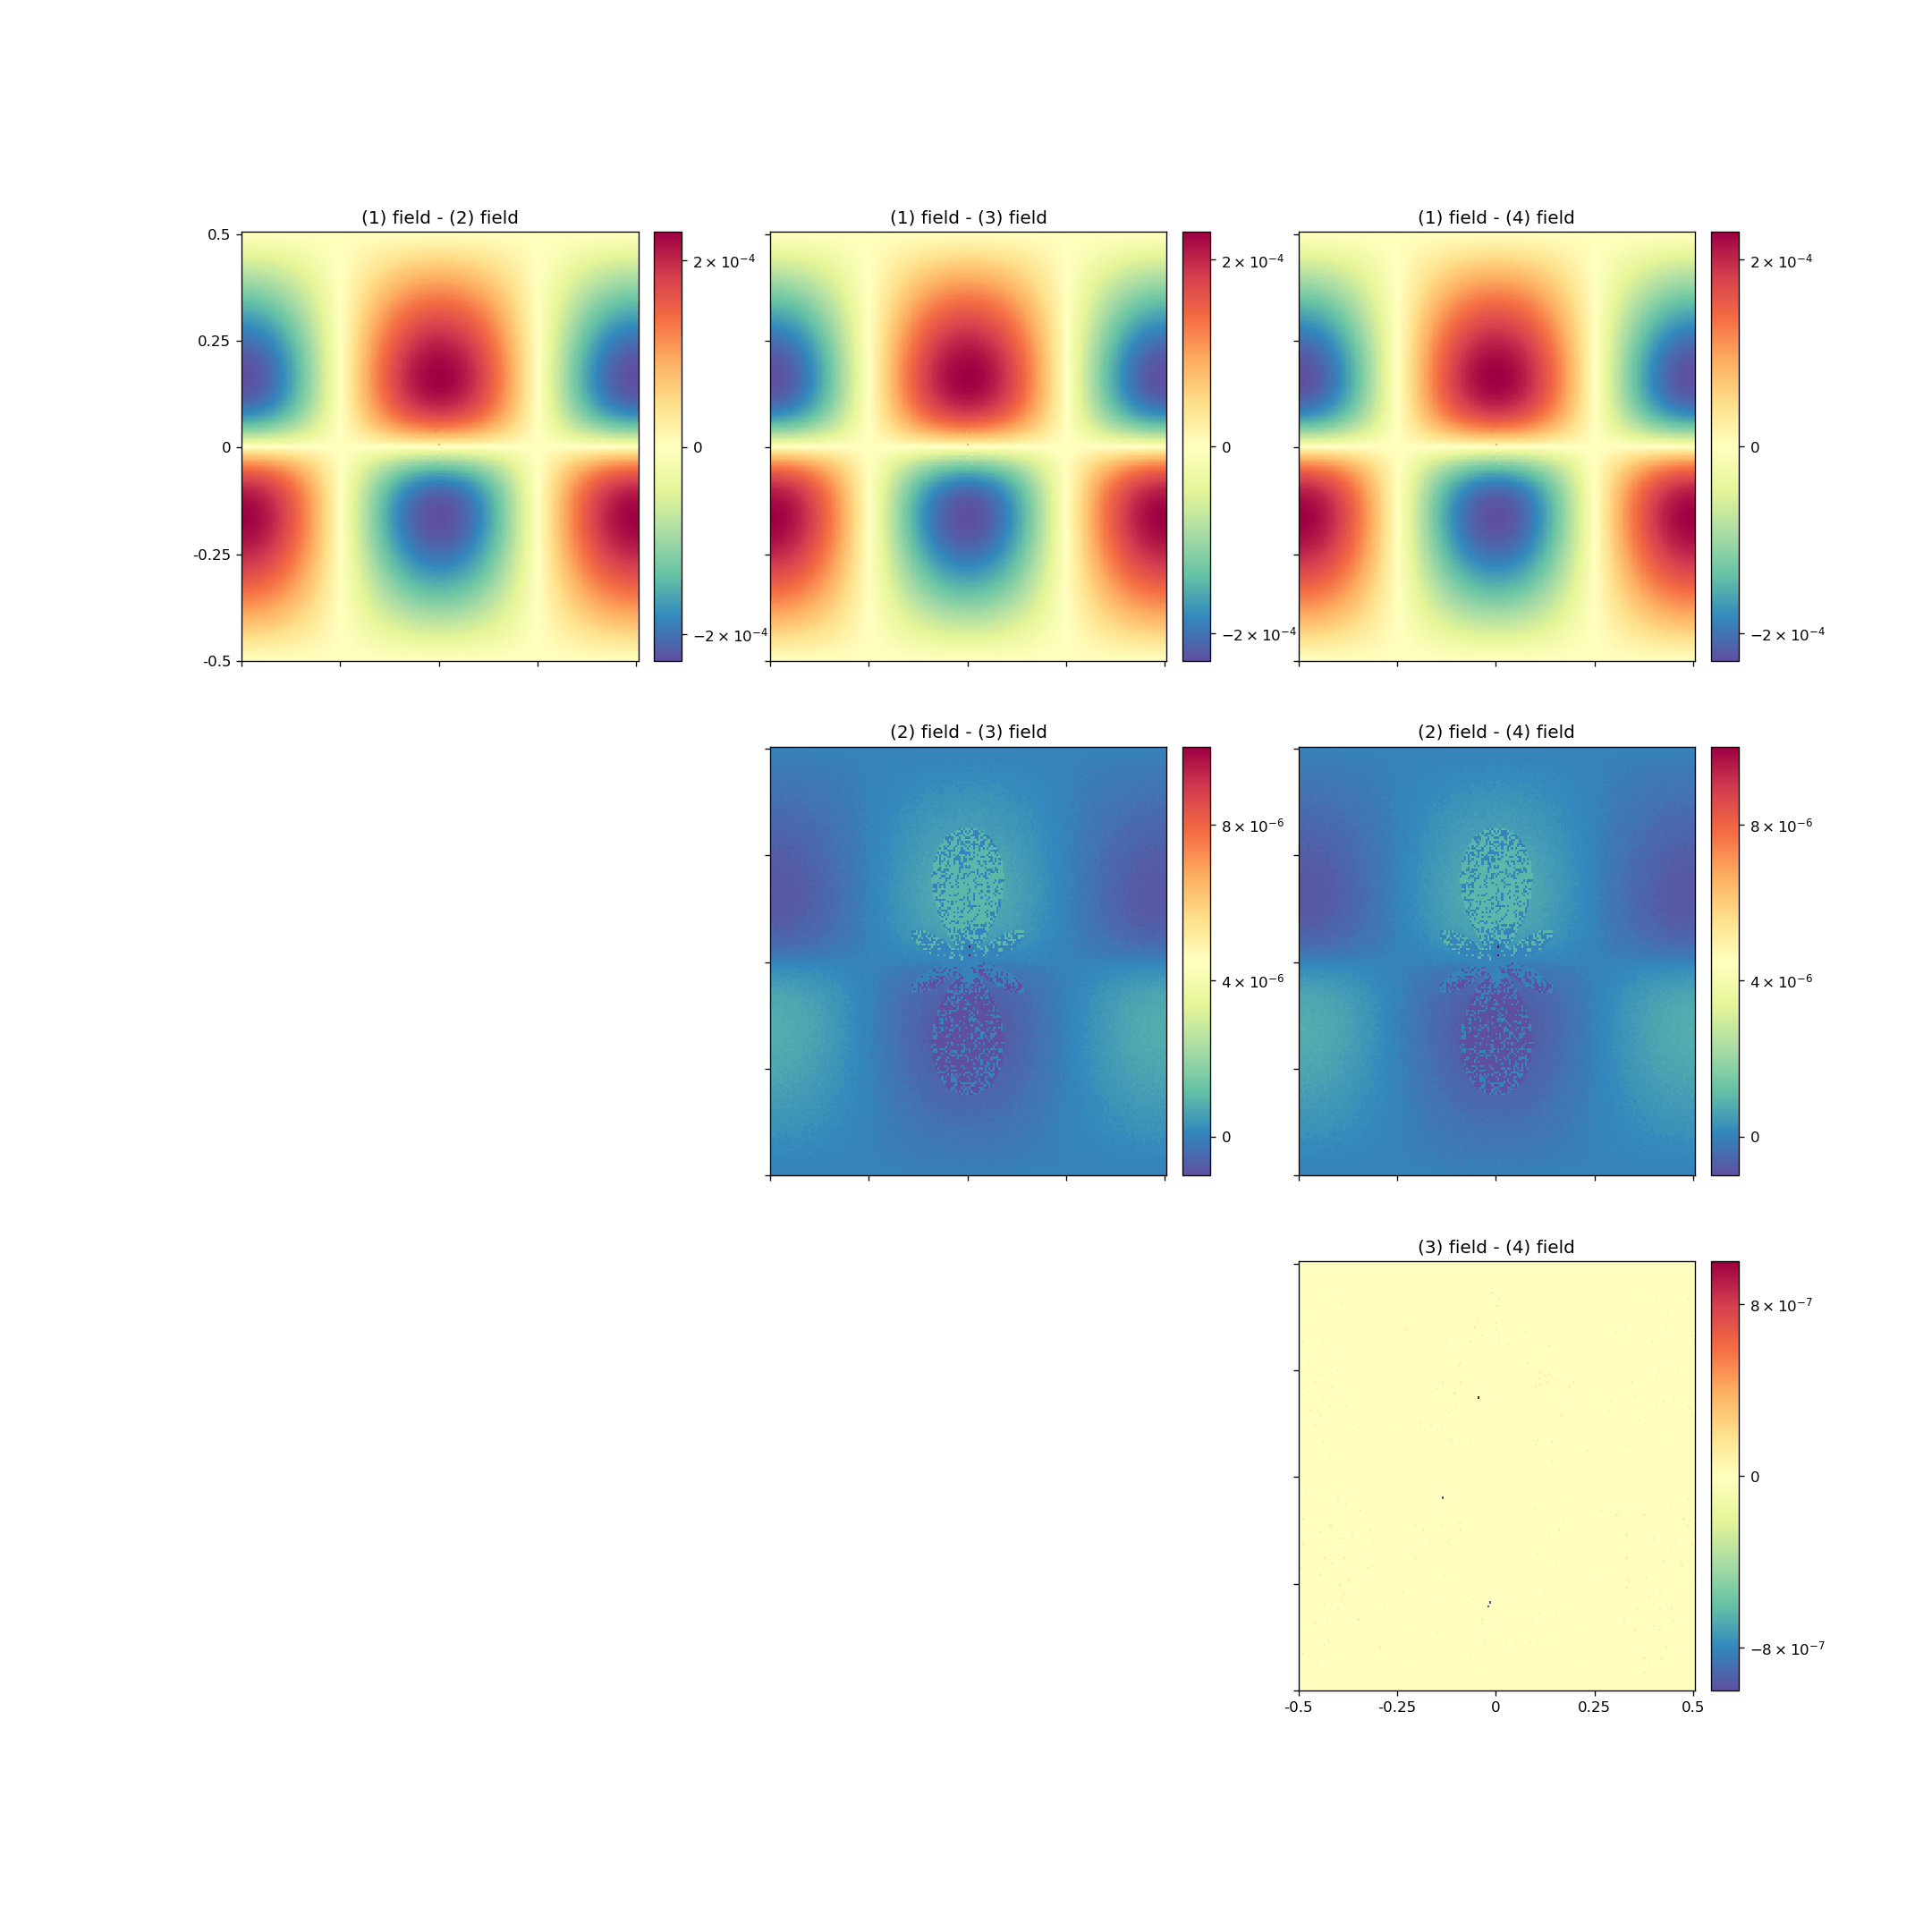
\includegraphics[width=.8\textwidth]{../difference_of_analytic_fields.png}
\end{figure}

\par Where row - column ordering is created. It can be seen that the very last plot,
that shows the difference between the 3rd and 4th analytic fields, where N=4 or N=3.
It can be clearly seen that disregarding some points the analytic fields become equal from N=3
and therefore the difference is almost everywhere zero.

\vspace{1cm}

\par Having plotted the difference of analytic fields I moved on with
showing the differences of analytic and ELTE code-named stress fields.

\begin{figure}[H]
	\centering
	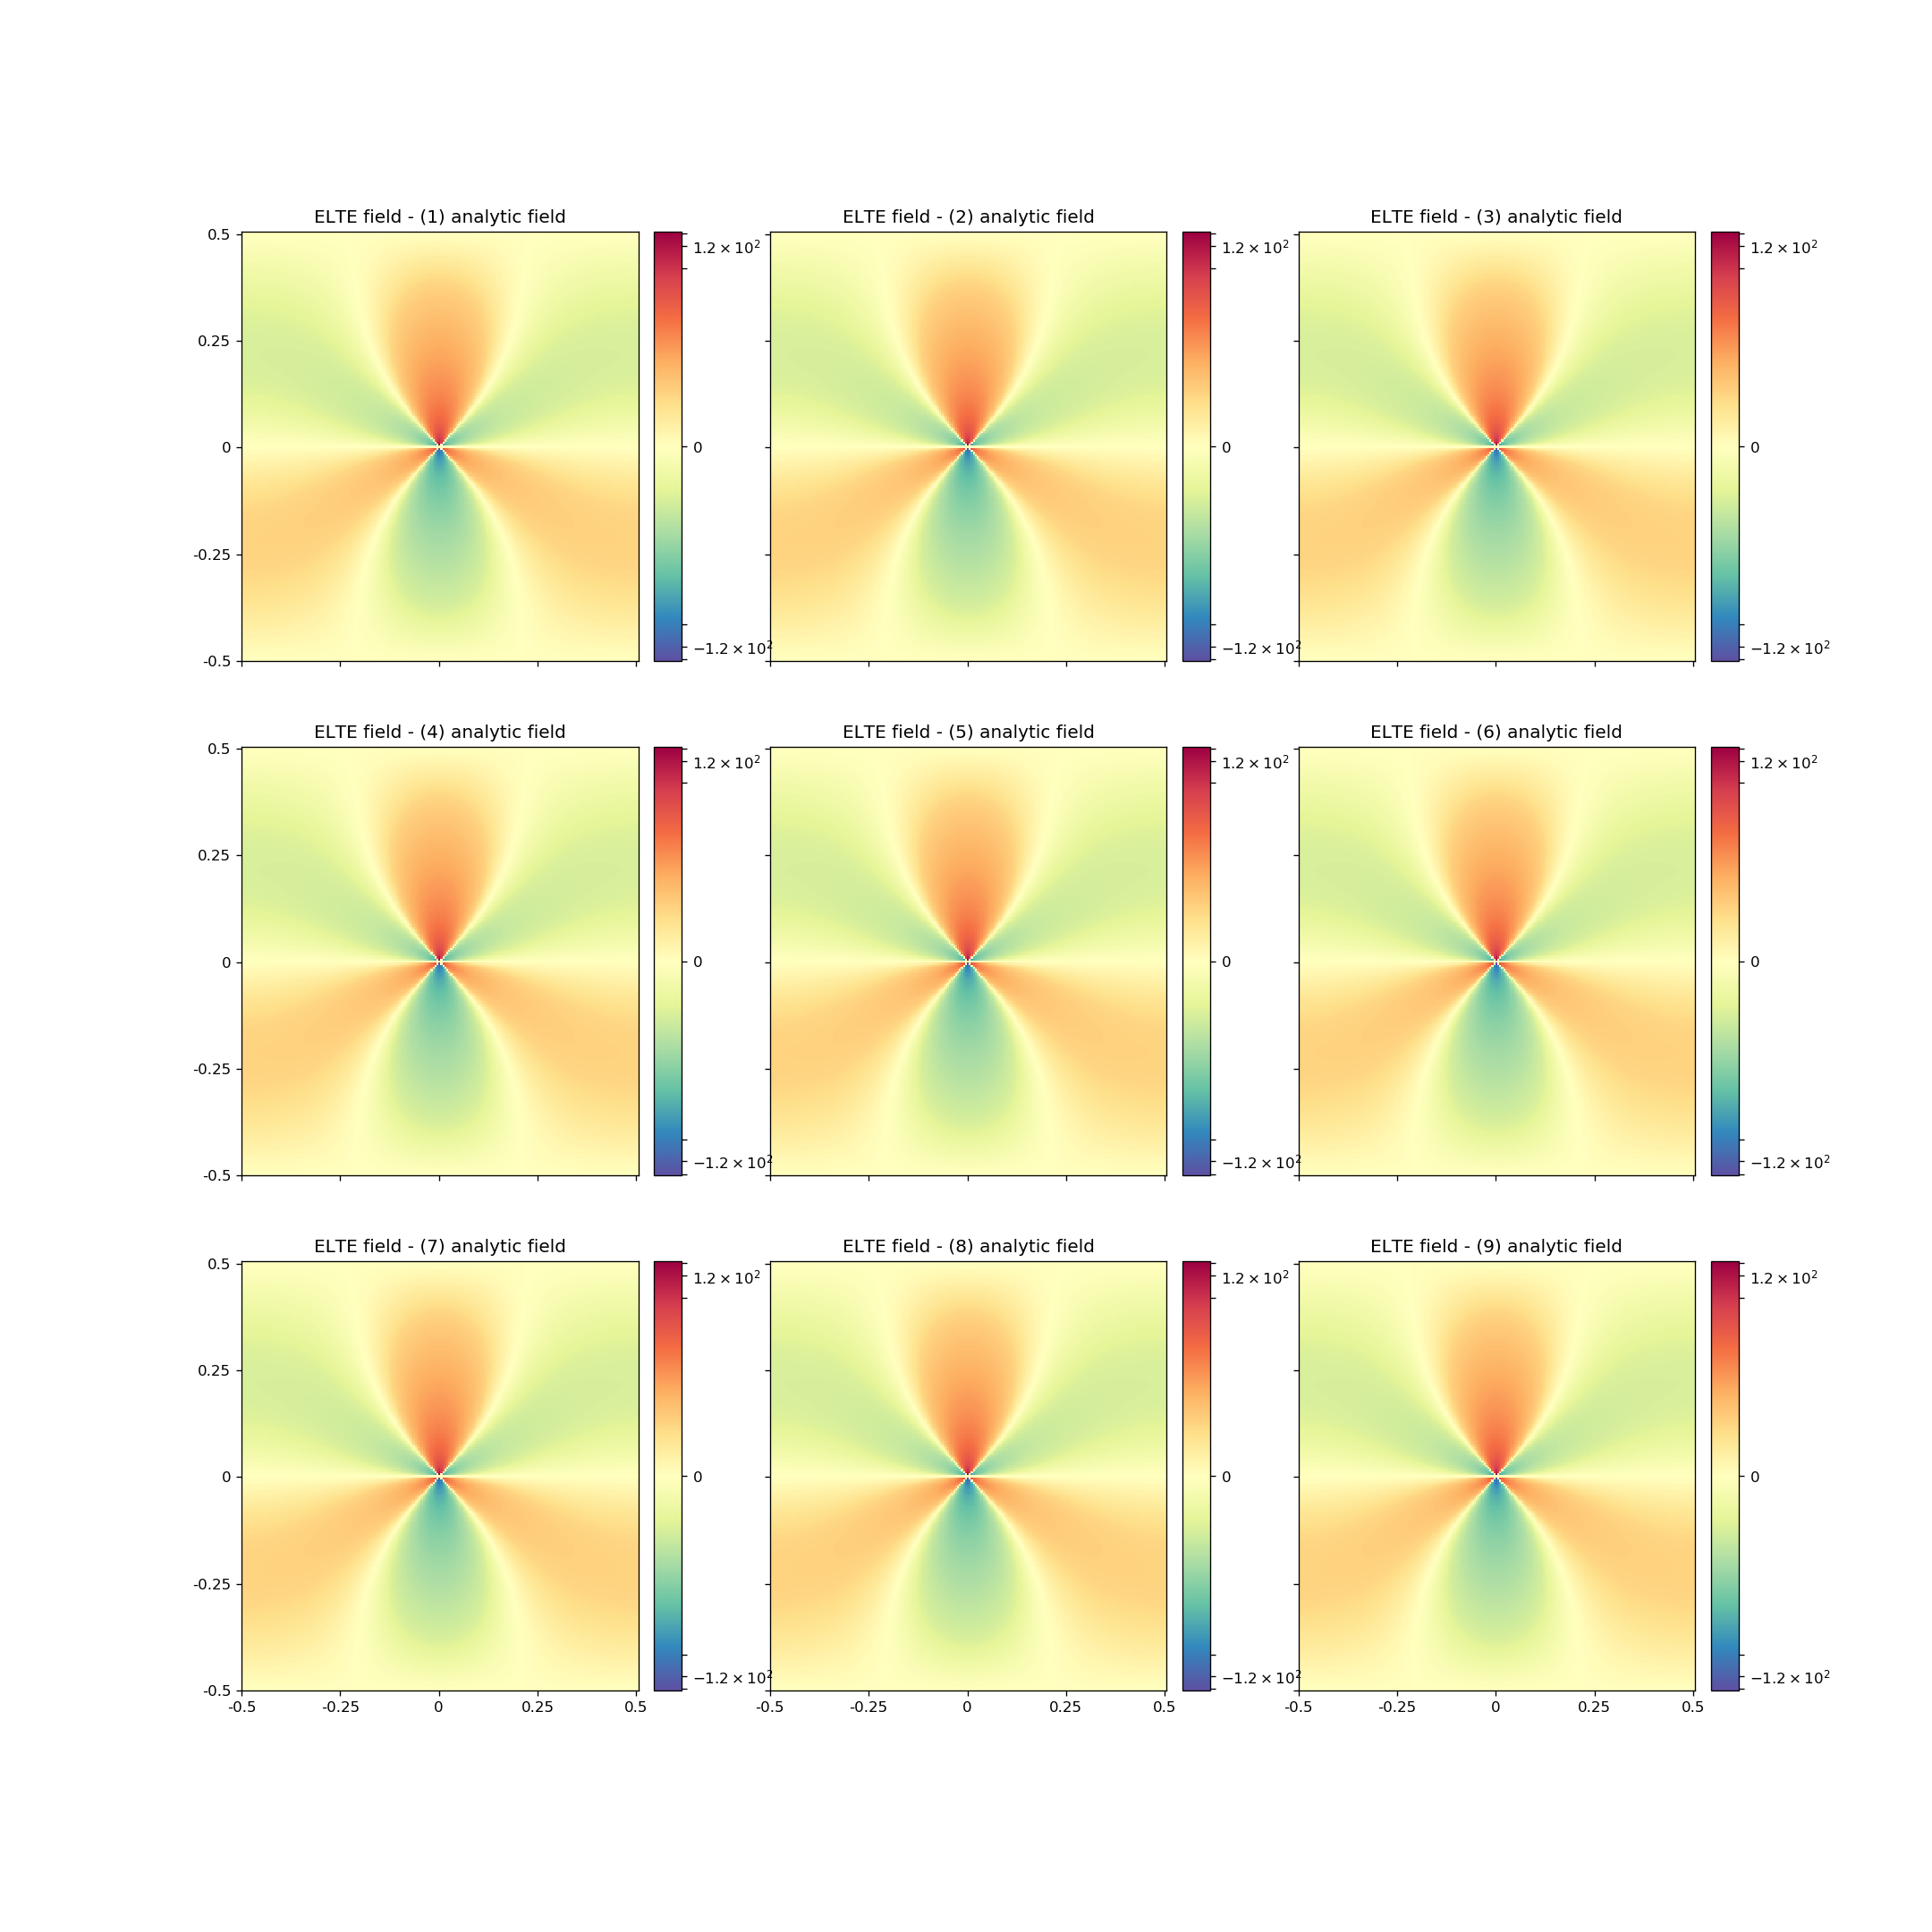
\includegraphics[width=.8\textwidth]{../difference_of_analytic_field_and_elte_field.png}
\end{figure}

\par From this plot it can be derived that they are equal almost everywhere but in the middle where
the differences are significant.

\end{document}